\documentclass[14pt]{beamer}
% \useoutertheme{miniframes}

\usepackage{ngerman}
\usepackage[utf8]{inputenc}
\usepackage[T1]{fontenc}
\usepackage{textcomp}
% \usepackage{amsmath,amsfonts,amssymb}
\usepackage{url}

% disable Navigation at the bottom
\beamertemplatenavigationsymbolsempty

% page numbers
% \setbeamertemplate{footline}[frame number]
% \setbeamertemplate{footline}
\setbeamertemplate{headline}

% style for source code
\usepackage{listings}
\newcommand{\Hilight}{\makebox[0pt][l]{\color{light-gray}\rule[-4pt]{1.0\linewidth}{12pt}}}
\usepackage[framed,numbered]{mcode}
\usepackage{color}
\definecolor{light-gray}{gray}{0.80}
  
% use {\mono lorem} to set something in monospace
\newcommand{\mono}[1]{\ttfamily\fontsize{14}{14}\selectfont #1}

% wanna use Metapost?
\makeatletter
\newcommand\@ptsize{12}
\makeatother

\usepackage{mflogo}
\usepackage{emp}
\DeclareGraphicsRule{*}{mps}{*}{}


\title{\LaTeX{} Beamerclass Presentation\\Template}   
\author{Max Mustermann} 
\date{\today} 


%===================================
\begin{document}

\frame{\titlepage} 

\frame{\frametitle{Table of contents}\tableofcontents} 


%===================================
\section{Introduction} 
\subsection{About Me}

\frame{\frametitle{About Me} 
	\begin{itemize}
		\item Who am I?\\ \ \\
		
		\item \url{http://github.com/cmichi}
	\end{itemize}
}


\frame{\frametitle{What is this about?} 
	\begin{figure}[ht]
		\centering{
			\Large Creative Coding
		}
	\end{figure}
}


\frame{\frametitle{Centered Image} 
	\begin{figure}[ht]
		\centering{
			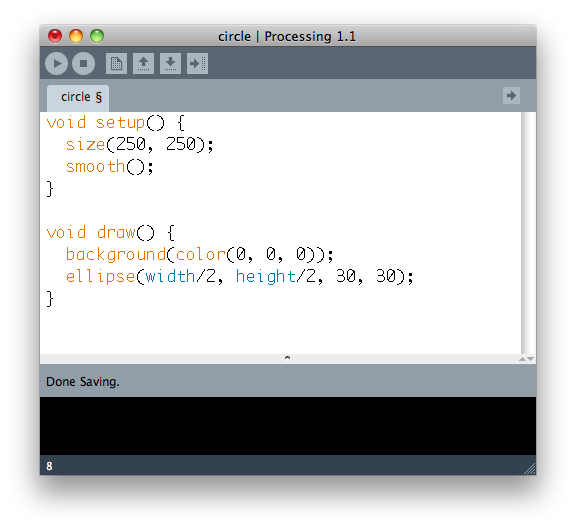
\includegraphics[scale=.45]{content/processing.png}
		}
	\end{figure}
}


\frame{\frametitle{Large Image}
	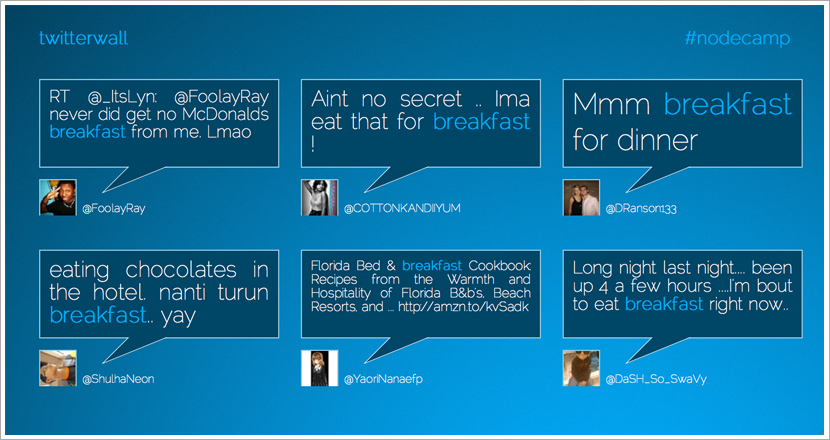
\includegraphics[scale=.38]{content/twitterwall.png}
	
	\vfill
	\hfill\scriptsize{Source: \url{https://github.com/cmichi/twitterwall}}	
}


%===================================
\section{Content} 
\subsection{First Content}
\frame{\frametitle{Some stuff}
	\begin{itemize}
		\item Code
		\item Algorithmen entwerfen
		\item Parameter \& Codeanpassung
		\item Archtitektur, Produktdesign
	\end{itemize} 
}


\frame{\frametitle{API}
	\begin{itemize}
		\item 2D / 3D Primitives
		\item PFont, PImage, \dots{}
		\item Input, Output\\ \ \\ 
		
		\item + enorm viele Librarys
		\item + viele Beispiele
	\end{itemize} 
}



\begin{frame}[fragile]
	\frametitle{Some Code}

	\begin{lstlisting}[language=Java, frame=single,
				% width of the box: linewidth=6.5cm, 
				basicstyle=\ttfamily\fontsize{10}{12}\selectfont,
				escapechar=\%]
		%\Hilight%void setup() 
		{
		  size(250, 250); 
		  smooth();
		}
				
		void draw() 
		{
		  background(0);
		  ellipse(width/2, height/2, 
		          30, 30);
		}		
	\end{lstlisting}	
\end{frame}


\begin{frame}[fragile]
	\frametitle{Some Code}

	\begin{lstlisting}[language=Java, frame=single,
				basicstyle=\ttfamily\fontsize{10}{12}\selectfont,
				escapechar=\%]
		void setup() 
		{
		%\Hilight%  size(250, 250); 
		  smooth();
		}
				
		void draw() 
		{
		  background(0);
		  ellipse(width/2, height/2, 
		          30, 30);
		}		
	\end{lstlisting}	
\end{frame}



\begin{frame}[fragile]
	\frametitle{\MP}
	\begin{figure}[ht]
		\centering{
			\includegraphics{content/house.mps}
		}
	\end{figure}
\end{frame}


\frame{\frametitle{}
	\begin{figure}[ht]
		\centering{
			\Large{\texttt{\$ traceroute}}
		}
	\end{figure}
}

\frame{\frametitle{Was brauchen wir?}
	\begin{itemize}
		\item Stream: {\mono traceroute} nach Processing		
		\item Separater Thread im Hauptprogramm
	\end{itemize} 
}


\frame{\frametitle{}
	\begin{figure}[ht]
		\centering{
			\Large{Website $\rightarrow$ Dynamische Datenstruktur}
		}
	\end{figure}
}


\frame{\frametitle{Wikileaks}
	\begin{itemize}
		\item 28. November 2010: Diplomatic cable release
		\item 2. Dezember 2010: EveryDNS\\ \ \\		
		
		\item ``\textit{Wikileaks is currently under heavy attack.}''
	\end{itemize}
}


%===================================
\section{The End}
\frame{\frametitle{Weiterführendes} 

	\begin{block}{Online}
	\begin{itemize}
		\item \url{http://processing.org/reference}
		\item \url{http://nodejs.org}
	\end{itemize}
	\end{block}

	\begin{block}{Bücher}
	\begin{itemize}
		\item Generative Gestaltung: Entwerfen. Programmieren. Visualisieren.
		\item The OpenGL Programming Guide
	\end{itemize}
	\end{block}
}

\frame{\frametitle{Software used} 
	\begin{block}{Umgebung}
		Mac OS X, vim
	\end{block}

	\begin{block}{Satz}
		\LaTeX{} beamer
	\end{block}

	\begin{block}{Grafiken}
		METAPOST
	\end{block}
	
	\vfill
	Slides are available on \url{http://github.com/cmichi}
}


\end{document}

